\documentclass[12pt]{article}
\raggedbottom

\usepackage[utf8]{inputenc}
\usepackage{graphicx}
\usepackage[english]{babel}
\usepackage{csquotes}
\usepackage{lipsum}
\usepackage{fancyhdr}
\usepackage{pdfpages}
\usepackage{wrapfig}
\usepackage{siunitx}
\usepackage{subcaption}
\usepackage{float}
\usepackage{enumitem}
\usepackage{subcaption}
\usepackage{framed}
\usepackage{listings,xcolor}
\usepackage{inconsolata}
\usepackage{setspace}
\usepackage[T1]{fontenc}
\usepackage[hidelinks]{hyperref}
\usepackage{booktabs}
\usepackage{amsmath}
\usepackage[backend=biber, sorting=none]{biblatex}
\usepackage[a4paper,width=160mm,top=25mm,bottom=25mm]{geometry}

\captionsetup{compatibility=false}
\definecolor{shadecolor}{gray}{0.8}
%\nocite{*}
\addbibresource{sources.bib}
\setcounter{biburllcpenalty}{7000}
\setcounter{biburlucpenalty}{8000}

\title{\textbf{\textsc{Assignment 1: Veracrypt}}\\Digital Forensics}

\author{Elisa Pioldi\\
        ID 12305812}
\date{October 25, 2023}

\begin{document}

\maketitle

\section{Factual part}

\subsection{Task}

The goal of this task was to recover the password of a \textbf{Veracrypt container} through a \textbf{bruteforce} attack.
The container encryption was performed with the cryptographic algorithm \textit{AES} with \textit{RIPEMD-160} as the hash function.

This report includes the analysis of multiple containers, to provide specific benchmarks.

\subsection{Containers analyzed}
\label{sec:containers}

I downloaded from the website \href{https://is.gd/mkveracrypt}{\texttt{is.gd/mkveracrypt}} the following containers, with input \texttt{12305812}:

\begin{itemize}
\item Lower case - 4 digits
\item Alpha - 4 digits
\item Alphanumeric - 4 digits
\item Special - 4 digits
\item Numbers - 4 digits
\item Numbers - 5 digits
\item Numbers - 8 digits
\end{itemize}

The reason for this choice is explained in the section \ref{sec:choice}.

\subsection{Containers hashes}

To verify the containers' integrity I computed just after the download of the SHA-1 checksum \cite{sha1} for each of them (see Table \ref{table:sha1}).

\begin{table}[!ht]
    \centering
    \begin{tabular}{ccc}
    \toprule
        \textbf{Character set} & \textbf{Length} & \textbf{SHA-1 checksum} \\ 
        \midrule
        Lower case & 4 & \texttt{8da0a7118fc2fedadb5714728435c4a1e03ec78c} \\ 
        Special & 4 & \texttt{cfcd5ee35c6729e88e0ff1b12c0ebdf80af6aa12} \\ 
        Alpha & 4 & \texttt{338d19ea6ab41ca770a92c0fd4d876cff746c3f3} \\ 
        Alphanumeric & 4 & \texttt{1fd07b016f56e9e4e3a3b8c9efa6d37684955b7b} \\ 
        Numbers & 4 & \texttt{265fcd87b60091d957be21cd6e39355c3918a191} \\ 
        Numbers & 5 & \texttt{5f670ad147cc2513dadf5e400ced2a4e7db9777d} \\ 
        Numbers & 8 & \texttt{21cdedf401ff1027885b6ee42c8b506bbc54e76e} \\ 
    \bottomrule
    \end{tabular}
    \caption{SHA-1 checksum for each container.}
    \label{table:sha1}
\end{table}

\subsection{Software and hardware specifications}
\label{sec:specs}

For this analysis, I utilized the following software:

\begin{itemize}
    \item \textbf{Veracrypt} \cite{veracrypt} -- version 1.24 (update 7); to perform container mounting and access.
    \item \textbf{Hashcat} \cite{hashcat} -- version 6.2.6; the world's fastest password cracker, used to find containers' passwords through brute force. Hashcat provides a specific mode to attack the container's encryption \cite{hc-modes}; moreover, I exploited its GPU optimization on the graphic card GTX 1060 (6 GB of VRAM), choosing a moderate workload profile for its execution. 
\end{itemize}

\begin{figure}[!ht]
     \centering
     \begin{subfigure}[b]{0.5\textwidth}
         \centering
         
\includegraphics[width=\textwidth]{images/hashcat.png}.
         \label{fig:hashcat}
     \end{subfigure}
     \hspace{30 pt}
     \begin{subfigure}[b]{0.3\textwidth}
         \centering
         
\includegraphics[width=\textwidth]{images/veracrypt.png}.
    \label{fig:veracrypt}
     \end{subfigure}
\end{figure}

\subsection{Password cracking}

After the preliminary analysis, I ran Hashcat on every downloaded container to collect statistics and passwords.

You can see some of the statistics (such as execution time and number of hashes/second) concerning simple character sets in Table \ref{table:stats}. For better understanding of time behavior, see Section \ref{sec:time}.

\begin{table}[!ht]
    \centering
    \begin{tabular}{cccc}
    \toprule
        \textbf{Character set} & \textbf{Length} & \textbf{Time} & \textbf{Hashrate}\\ 
        \midrule
        Numbers & 4 & 26 secs & 397 H/s \\ 
        Numbers & 5 & 1 min, 9 secs & 363 H/s \\ 
        Lower case & 4 & 12 mins, 37 secs & 411 H/s \\ 
    \bottomrule
    \end{tabular}
    \caption{Statistics of some cracked containers.}
    \label{table:stats}
\end{table}

For every execution, the hashrate (number of hashes per second) was around 400 H/S average (for hardware benchmarks, see Section \ref{sec:specs}). I couldn't crack the container with the numeric password of length 8, since it would have required around 3 days, according to Hashcat's estimation.

After collecting all the passwords I could mount every Veracrypt container to check the content inside. All the recovered passwords are shown in Table \ref{table:pwd}.

\begin{table}[!ht]
    \centering
    \begin{tabular}{ccc}
    \toprule
        \textbf{Character set} & \textbf{Length} & \textbf{Password} \\ 
        \midrule
        Lower case & 4 & \texttt{yxgy}  \\ 
        Special & 4 & \texttt{=!(;}\\ 
        Alpha & 4 & \texttt{kDfl} \\ 
        Alphanumeric & 4 & \texttt{EvXY} \\ 
        Numbers & 4 & \texttt{2709} \\ 
        Numbers & 5 & \texttt{83450} \\ 
    \bottomrule
    \end{tabular}
    \caption{Recovered passwords for each container.}
    \label{table:pwd}
\end{table}

\subsection{Container contents}

Every container contains four different files: three pictures (Figure \ref{fig:awesome}, \ref{fig:trippin} and \ref{fig:wasted}) and one text file. 

\begin{figure}[H]
    \begin{center}
    
\includegraphics[width=0.9\textwidth]{images/awesome.jpg}
    \caption{First picture stored in the container (awesome.jpg).}
    \label{fig:awesome}
    \end{center}
\end{figure}

\begin{figure}[H]
     \centering
     \begin{subfigure}[b]{0.46\textwidth}
         \centering
         
\includegraphics[width=\textwidth]{images/trippin.jpg}
         \caption{trippin.jpg}
         \label{fig:trippin}
     \end{subfigure}
     \begin{subfigure}[b]{0.45\textwidth}
         \centering
         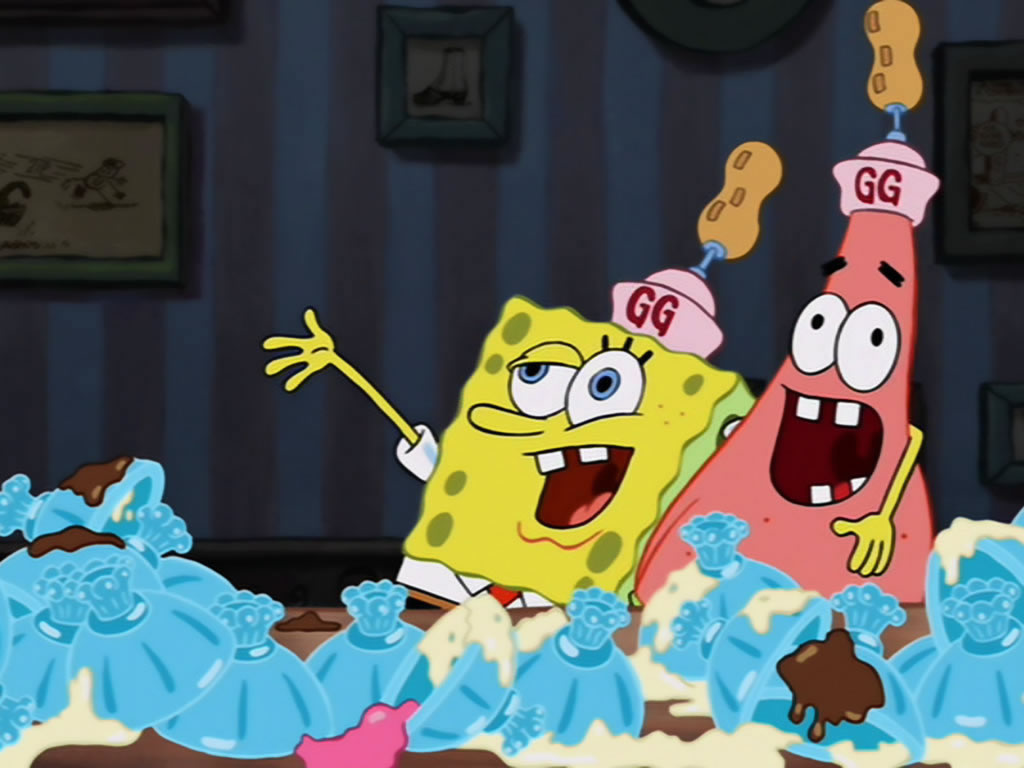
\includegraphics[width=\textwidth]{images/wasted.jpg}
         \caption{wasted.jpg}
         \label{fig:wasted}
     \end{subfigure}
     \caption{Last two pictures stored in the container.}
\end{figure}

Each text file, named \texttt{secret.txt}, contains a \textbf{42-character long string} (see Table \ref{table:secret}), slightly different from container to container.

\begin{table}[!ht]
    \centering
    \begin{tabular}{ccc}
    \toprule
        \textbf{Character set} & \textbf{Length} & \textbf{Secret} \\ 
        \midrule
        Lower case & 4 & \texttt{fede1cea08a6465514160a54076874f2c967ffc53b} \\ 
        Special & 4 & \texttt{fede1cea08a6465514160d54076874f2c967ffc53b} \\ 
        Alpha & 4 & \texttt{fede1cea08a6465514160e54076874f2c967ffc53b} \\ 
        Alphanumeric & 4 & \texttt{fede1cea08a6465514160f54076874f2c967ffc53b} \\ 
        Numbers & 4 & \texttt{fede1cea08a6465514160c54076874f2c967ffc53b} \\ 
        Numbers & 5 & \texttt{fede1cea08a6465514161c54076874f2c967ffc53b} \\ 
    \bottomrule
    \end{tabular}
    \caption{Secrets inside each container.}
    \label{table:secret}
\end{table}

\section{Expert testimony}

\subsection{Background}

\subsubsection{Containers choice}
\label{sec:choice}

Since cracking passwords is computationally demanding, I had to choose by selecting which containers to analyze. I wanted to have a significant pool in matters of time benchmarks, passwords and revealed contents. 

Since numeric passwords are easy to crack, I looked for 3 different containers with passwords of 4, 5 and 8 digits, to have an overview of benchmarks when changing the password length. I already knew evaluating my hardware benchmark would have been infeasible, but I wanted to see how much computational time Hashcat would have estimated. Moreover, since the number of lower case and upper case letters are the same, I chose to analyze only one container with such passwords.

All of the reasons above led me to choose the ones specified in Section \ref{sec:containers}.

\subsubsection{Hashrate}

I chose to use the Hashcat workload profile 3 (out of 4). Still, nonetheless, the hashrate was very low (only hundreds of hashes per second) compared to the most classical hashing algorithms (in order of thousands of MH/s) \cite{hc-benchmarks}. I checked various benchmarks and all the Veracrypt ones showed this behaviour. 

This is evidence of how well-resistant Veracrypt is against brute-force attacks.

\subsection{Secrets analysis}

The \textit{secrets} reported in Table \ref{table:secret} seem to present some specific pattern.

The differences in the secrets only concern two characters in the middle of the string: we have the same 20 characters, 2 specific digits and the same other 20 characters. Since SHA-1 produces a message digest of 40 characters \cite{sha1}, I supposed the first and the last characters in the secret are a sort of checksum of the input ID and something else. Concerning the central two digits, I noticed a recurring pattern: the first digits indicate the length of the password (0 for a 4 digits long password, 1 for a 5 digits long password and so on) and the last digits refer to the character set (\textit{a} for lower case, \textit{c} for numbers and so on).

\subsection{Strength analysis}

At this point, we have all the data to perform a password strength analysis. In particular, I elaborated two formulas to find two specific quantities, always concerning a \textbf{brute-force attack}: the maximum amount of time needed to crack a password and the minimum password length to resist for a given period. 

All the following computations are done considering a hashrate of 400 H/s for the previous tests with Hashcat.

\subsubsection{Maximum cracking time}
\label{sec:time}

First, let's find a way to compute how much time is needed to brute-force any container.

Given $S$ the character set (for instance, $|S|=26$ if we choose the set of lowercase letters), $l$ the password length and $hps$ the number of hashes per second, time (maximum number of seconds, i.e. upper bound) is computed as follows:

\[time = \frac{|S|^l}{hps}\]

Through this formula, we can compute for instance the cracking time for a 4, 5 and 6-digit password (I'll consider these amounts of digits to show the exponential growth in comparison to the 4-digit passwords used previously for tests). Results are displayed in Table \ref{table:time}.

\begin{table}[!ht]
    \centering
    \begin{tabular}{lcc}
    \toprule
        \textbf{Character set} & \textbf{Set cardinality} & \textbf{Time} \\ 
        \midrule
        \textbf{4 digits} \\
        Numbers & 10 & 25 seconds \\
        Special & 17 & 3 minutes \\ 
        Lower case / Upper case & 26 & 19 minutes \\ 
        Alpha & 52 & 5 hours \\ 
        Alphanumeric & 62 & 10 hours \\ 
        Full & 79 & 27 hours \\ 
        \midrule
        \textbf{5 digits} \\
        Numbers & 10 & 4 minutes \\
        Special & 17 & 1 hour \\ 
        Lower case / Upper case & 26 & 8 hours \\ 
        Alpha & 52 & 11 days \\ 
        Alphanumeric & 62 & 26 days \\ 
        Full & 79 & 89 days \\ 
        \midrule
        \textbf{6 digits} \\
        Numbers & 10 & 41 minutes \\
        Special & 17 & 16 hours \\ 
        Lower case / Upper case & 26 & 8 days \\ 
        Alpha & 52 & 11 days \\ 
        Alphanumeric & 62 & 1.5 years \\ 
        Full & 79 & 19 years \\ 
    \bottomrule
    \end{tabular}
    \caption{Maximum amount of time to crack passwords of different lengths with hashrate of 400 H/s.}
    \label{table:time}
\end{table}

As we could expect, time grows exponentially with the character set's cardinality; moreover, note that this is just an upper bound: this explains why in the Hashcat tests I managed to recover passwords in less time (see Table \ref{table:stats}).

\subsubsection{Minimum password length}

Let's assume now we have to find a \textbf{10-year-resistant password} (I will consider for the calculation that in a year there are approximately $\num{3.156e7}$ seconds \cite{unit-converter}, therefore $\num{3.156e8}$ seconds in 10 years).

Given $S$ the character set and $hps$ the number of hashes per second, the length (minimum number of digits in the password, i.e. lower bound) is computed as follows:

\[length = \log_{|S|}{(\num{3.156e8} \times hps)}\] 

Using the formula above, we can easily compute how long our password has to be to resist a brute-force attack for 10 years, performed on hardware with the same specifications as mine (hashrate of 400 H/s). The results are shown in the Table \ref{table:10year}.

\begin{table}[!ht]
    \centering
    \begin{tabular}{lcc}
    \toprule
        \textbf{Character set} & \textbf{Set cardinality} & \textbf{Password length} \\ 
        \midrule
        Numbers & 10 & 11.1 \\
        Special & 17 & 9.0 \\ 
        Lower case / Upper case & 26 & 7.8 \\ 
        Alpha & 52 & 6.4 \\ 
        Alphanumeric & 62 & 6.1 \\
        Full & 79 & 5.8 \\
    \bottomrule
    \end{tabular}
    \caption{Minimum average length for a 10-year resistant password with hashrate of 400 H/s.}
    \label{table:10year}
\end{table}

\addcontentsline{toc}{chapter}{Sources}
\printbibliography[title={Sources}]

\end{document}
